\documentclass{article}
\usepackage[utf8]{inputenc}

\title{CS3110 Hnefatafl Design Doc}
\author{Elizabeth VanDenburgh (eav38), Joseph Dwyer (jmd456), Taeer Bar-Yam (tb442)}
\date{November, 12 2015}

\begin{document}

\maketitle

\section{Hnefatafl Game Dynamics}
The game is played on an $11\times 11$ checkered board with two uneven sides.
$12$ white pieces are positioned around a white ``king'' at the center of the
board, with $24$ black pieces arranged on the edges surrounding them.
See~\ref{fig:initial_position}.
\begin{figure}
  \label{fig:initial_position}
  \centering
    \scalebox{.5}{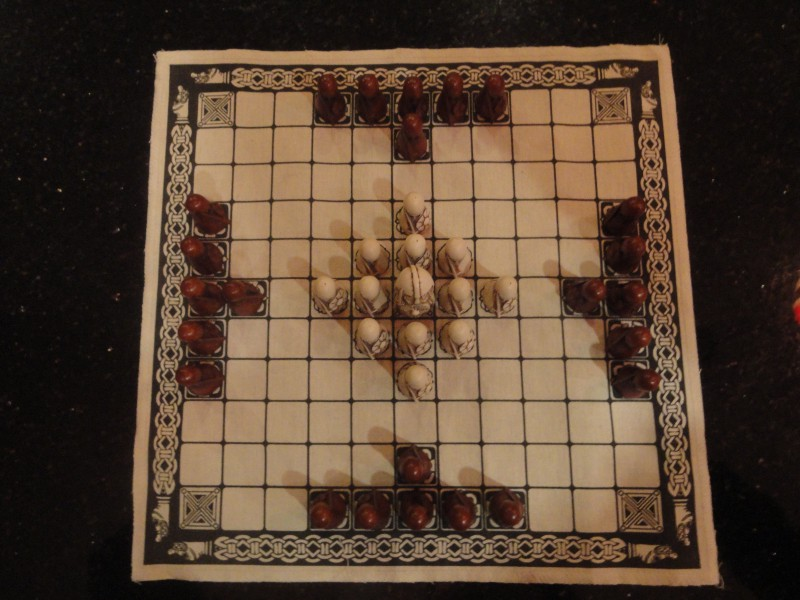
\includegraphics{hnefatafl}}
    \caption{Hnefatafl starting board position. Source: \url{https://medium.com/war-is-boring/you-have-to-play-this-1-600-year-old-viking-war-game-cef088ae4e2d\#.10kof827g}}
\end{figure}
There are three main mechanics involved in the game:
\begin{enumerate}
\item \textbf{Movement}\\
  Pieces move like rooks in chess (horizontally or vertically).
  Only the king has a limited motion of three squares at a time.
\item \textbf{Capturing}\\
  When a piece is flanked by two pieces of the opposing color, that piece is
  ``captured'' and is removed from the board.  This flanking must be done actively
  by the offense (i.e. the center piece can move between the others without
  being captured).\\
  The king cannot participate in flanking an opponent. In the case of the king,
  it must be flanked on all sides to be considered ``captured.''
\item \textbf{Winning}\\
  Black wins when the king is captured, or the king's only escape is to move
  back to the center square of the board.\\
  White wins when the king is moved to one of the side squares of the board.
\end{enumerate}
See: \url{https://en.wikipedia.org/wiki/Tafl\_games\#Hnefatafl}
\section{Interface:}
Ultimately we would like to implement the interface as a GUI using openGL, and
allow click-and-drag motion commands. Initially, we will implement a text-based
interface that uses chess-like notation for movement and output a ASCII grid to
show positions of pieces. This interface will likely remain available as an
option\\
This will be playable against another human player, or against an AI.
\section{Stretch Goals:}
\begin{itemize}
\item Hnefatafl is an old game, and there are many versions of it that exist.
  Time permitting, we would like to implement many of these variants, working
  off of a general game core.
\item Detect if the game has become unwinnable.
\end{itemize}

\section{Architecture}
Thinking pipe and filter
information goes from user - gui - backend - gui - user

\section{System Design}
\subsection{GUI}
\subsection{Backend}
Depends on GUI.
Depends on Menu.
Depends on Helpers.
\subsection{AI}
\subsection{Helpers}
Makes up for functions that should have been included in OCaml.
\subsection{GameType}
all types of things, maybe helper functions
most things will depend on it.

\section{Module Design}

\section{Data}
\begin{itemize}
\item Player turn
\item Piece locations to maintain the current board
\item Game configurations
\end{itemize}
Structures include:
\begin{itemize}
\item Piece types
\item Game configurations
\item Board with dimensions and piece locations
\end{itemize}

\section{External Libraries}
\begin{itemize}
\item Termbox for creating an ascii board
\item OpenGL for creating a more graphical gui
\end{itemize}

\section{Testing Plan}
\begin{itemize}
\item Write unit tests for sate of the board after certain moves
\item Watch the AI play against itself
\item Get play testers
\end{itemize}

\end{document}
